\documentclass[class=minimal,border=0pt]{standalone}
\usepackage{tikz}
\usetikzlibrary{calc,patterns,decorations.pathmorphing,decorations.markings}

\newcommand\YM{3}
\newcommand\XG{0}
\newcommand\xs{5}
\newcommand\kvw{0.5}

\begin{document}
\tikzstyle{mass} = [draw,rectangle,rounded corners=1mm,fill=green!20]
\tikzstyle{ground}=[fill,pattern=north east lines,draw=none,minimum width=0.75cm,minimum height=0.3cm]
\tikzstyle{spring}=[thick,decorate,decoration={zigzag,pre length=0.5cm,post length=0.5cm,segment length=6}]
\tikzstyle{damper}=[thick,decoration={markings,  
  mark connection node=dmp,
  mark=at position 0.5 with 
  {
    \node (dmp) [thick,inner sep=0pt,transform shape,rotate=-90,minimum width=15pt,minimum height=3pt,draw=none] {};
    \draw [thick] ($(dmp.north east)+(8pt,0)$) -- (dmp.south east) -- (dmp.south west) -- ($(dmp.north west)+(8pt,0)$);
    \draw [thick] ($(dmp.north)+(0,-5pt)$) -- ($(dmp.north)+(0,5pt)$);
  }
}, decorate]

\begin{tikzpicture}
    \coordinate (m0) at (\XG-\xs,\YM);
    \coordinate (m1) at (\XG,\YM);
    \coordinate (m2) at (\XG+\xs,\YM);
    \node[mass] at (m0) (mass0) {$m_{i-1}$};
    \node[mass] at (m1) (mass1) {$m_i$};
    \node[mass] at (m2) (mass2) {$m_{i+1}$};
    \node[ground,anchor=north] at (\XG-\xs,0) (ground0) {};
    \node[ground,anchor=north] at (\XG,0) (ground1) {};
    \node[ground,anchor=north] at (\XG+\xs,0) (ground2) {};
    
    
    \coordinate (kvT) at (0,2.5);
    \coordinate (kvTL) at (-\kvw,2.5);
    \coordinate (kvTR) at (\kvw,2.5);

    \coordinate (kvB) at (0,0.5);
    \coordinate (kvBL) at (-\kvw,0.5);
    \coordinate (kvBR) at (\kvw,0.5);

    \draw[spring] (kvBR) -- (kvTR);
    \draw[damper] (kvBL) -- (kvTL);

    \draw[] (kvT) -- (mass1);
    \draw[] (kvTL) -- (kvTR);

    \draw[] (ground-i) -- (kvB);
    \draw[] (kvBL) -- (kvBR);


    \draw[] (ground0.north west) -- (ground0.north east);
    \draw[] (ground1.north west) -- (ground1.north east);
    \draw[] (ground2.north west) -- (ground2.north east);

    \draw (\XG-\xs-1,\YM) -- (mass0);
    \draw (mass2) -- (\XG+\xs+1,\YM);

    \node[] at (\xs/2, 4) (membrane) {Membrane};
    \draw[decorate,decoration={brace},thick] m1 to m2;
    \node[] at (\xs/2, 2) (adhesion) {Adhesion};
    \draw[decorate,decoration={brace},thick] m1 to m2;


\end{tikzpicture}
\end{document}



\iffalse
\documentclass{article}
\usepackage{tikz}
\usetikzlibrary{calc,patterns,decorations.pathmorphing,decorations.markings}

\begin{document}

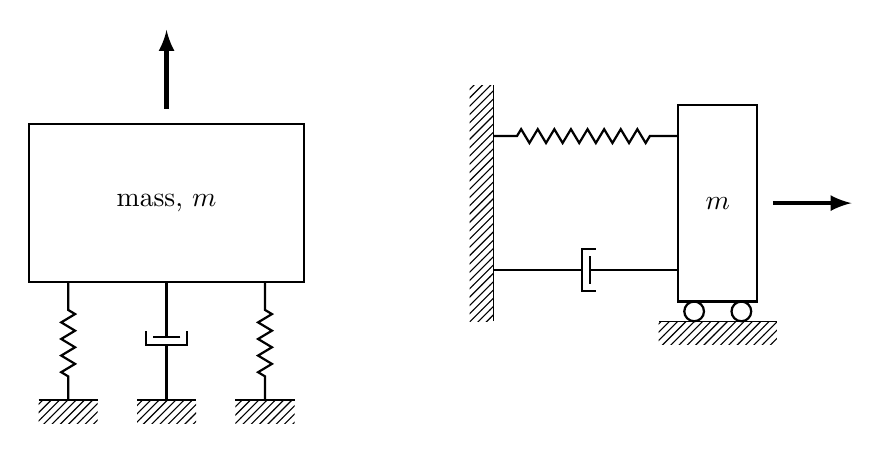
\begin{tikzpicture}[every node/.style={draw,outer sep=0pt,thick}]
\tikzstyle{spring}=[thick,decorate,decoration={zigzag,pre length=0.3cm,post length=0.3cm,segment length=6}]
\tikzstyle{damper}=[thick,decoration={markings,  
  mark connection node=dmp,
  mark=at position 0.5 with 
  {
    \node (dmp) [thick,inner sep=0pt,transform shape,rotate=-90,minimum width=15pt,minimum height=3pt,draw=none] {};
    \draw [thick] ($(dmp.north east)+(2pt,0)$) -- (dmp.south east) -- (dmp.south west) -- ($(dmp.north west)+(2pt,0)$);
    \draw [thick] ($(dmp.north)+(0,-5pt)$) -- ($(dmp.north)+(0,5pt)$);
  }
}, decorate]
\tikzstyle{ground}=[fill,pattern=north east lines,draw=none,minimum width=0.75cm,minimum height=0.3cm]


\node (M) [minimum width=3.5cm,minimum height=2cm] {mass, $m$};

\node (ground1) at (M.south) [ground,yshift=-1.5cm,xshift=-1.25cm,anchor=north] {};
\draw (ground1.north west) -- (ground1.north east);
\draw [spring] (ground1.north) -- ($(M.south east)!(ground1.north)!(M.south west)$);

\node (ground2) at (M.south) [ground,yshift=-1.5cm,anchor=north] {};
\draw (ground2.north west) -- (ground2.north east);
\draw [damper] (ground2.north) -- ($(M.south east)!(ground2.north)!(M.south west)$);

\node (ground3) at (M.south) [ground,yshift=-1.5cm,xshift=1.25cm,anchor=north] {};
\draw (ground3.north west) -- (ground3.north east);
\draw [spring] (ground3.north) -- ($(M.south east)!(ground3.north)!(M.south west)$);

\draw [-latex,ultra thick] (M.north) ++(0,0.2cm) -- +(0,1cm);

\begin{scope}[xshift=7cm]
\node (M) [minimum width=1cm, minimum height=2.5cm] {$m$};

\node (ground) [ground,anchor=north,yshift=-0.25cm,minimum width=1.5cm] at (M.south) {};
\draw (ground.north east) -- (ground.north west);
\draw [thick] (M.south west) ++ (0.2cm,-0.125cm) circle (0.125cm)  (M.south east) ++ (-0.2cm,-0.125cm) circle (0.125cm);

\node (wall) [ground, rotate=-90, minimum width=3cm,yshift=-3cm] {};
\draw (wall.north east) -- (wall.north west);

\draw [spring] (wall.170) -- ($(M.north west)!(wall.170)!(M.south west)$);
\draw [damper] (wall.10) -- ($(M.north west)!(wall.10)!(M.south west)$);

\draw [-latex,ultra thick] (M.east) ++ (0.2cm,0) -- +(1cm,0);
\end{scope}
\end{tikzpicture}

\end{document}
\usepackage{amsmath}
\usetikzlibrary{arrows}
\usetikzlibrary{decorations.pathreplacing}
\usetikzlibrary{backgrounds}
\usetikzlibrary{fit}

\begin{document}


\tikzstyle{Scyto} = [draw,thick,rounded corners=1mm]
\tikzstyle{MAPKpp} = [draw,thick,  fill=green!20]
\tikzstyle{arrow} = [->,thick,font=\fontsize{8}{8}]
\tikzstyle{Stot} = [rectangle, fill=gray!10, inner sep=0.4cm, rounded corners = 5mm, draw=black!50, dashed]

\begin{tikzpicture}[inner sep=2mm,>=stealth']
  %\draw[help lines] (-4,-4) grid (4,1);
  %\fill (0,0) circle (2pt) {};

  \node[Scyto, fill=blue!10] at (-2.5, 1) (Scyto) {$S_{cyto}$};
  \node[Scyto, fill=blue!10] at ( 2.5, 1) (Smem)  {$S_{mem}$};
  \node[Scyto, fill=blue!30] at (   0,-1) (Sves)  {$S_{ves}$};
  \node[fill=gray!10]        at (   0,-0.1) (Stot) {\textbf{S}$_{tot}$};
  \node[MAPKpp] at ( 0,-3.0) (MAPKpp) {MAPK$_{pp}$};
  \begin{pgfonlayer}{background}
    \node [Stot, fit=(Scyto) (Smem) (Sves)] {};
  \end{pgfonlayer}

  \draw[arrow] (Scyto.10) -- (Smem.170)  node[midway,above] {$p_1  = p_1(\mathit{Input})$}; 
  \draw[arrow] (Smem.190) -- (Scyto.350) node[midway,below] {$p_2$}; 
  \draw[arrow] (Smem)      .. controls +(down:1.3cm) and +(right:1.0cm) .. (Sves.east) node[auto,midway] {$p_3 = p_3(\mathit{S_{mem}})$};
  \draw[arrow] (Sves.west) .. controls +(left:1.0cm) and +( down:1.3cm)  .. (Scyto) node[midway,auto,fill=red!10] {$p_4 = p_4(x,\mathbf{S_{ves}}, \mathit{dS_{ves}})$};
  \draw[arrow] (Sves) -- (MAPKpp);
\end{tikzpicture}


  \draw[arrow] (Scyto.10) -- (Smem.170) node[midway,above] {$
    \begin{aligned} 
      dose &= grad*maxdose*(l+dX *x) \\
      p_1  &= p_5 * dose
    \end{aligned}
      $}; 

\end{document}

\fi
